\chapter{Método de pesquisa}
\label{cap:metodologia}

COLOCAR INTRODUCAO

\section{Introdução}

Nesta pesquisa proporemos um modelo para a estimação dos juros da dívida técnica em projetos de desenvolvimento de software. Nesse modelo, consideramos os juros como a variação negativa, na produtividade do projeto, causada pela existência da dívida técnica. Conforme ilustrado na Figura \ref{fig:cap_metodo_niveis_abstracao}, esse modelo possui dois níveis de abstração. O primeiro é conceitual e basea-se em uma definição abstrata tanto da produtividade de um projeto quanto do principal da dívida técnica. No segundo nível, já há uma definição das métricas que serão utilizadas para a estimação dos juros em projetos reais. O segundo nível de abstração é na verdade uma instância do modelo de primeiro nível. Futuramente podem ser definidas diversas instâncias do modelo de primeiro nível, cada uma terá de ser criada de acordo com as características dos projetos que serão avaliados. Por exemplo, em uma situação onde deseja-se estimar os juros da dívida técnica de um projeto web provavelmente serão utilizadas métricas de produtividade diferentes das métricas de um projeto de software. No Capítulo \ref{estimacao:juros} forneceremos  uma definição precisa a respeito do modelo de estimação dos juros e seus níveis de abstração. 

Para avaliarmos a aplicabilidade tanto do modelo de primeiro nível quanto de segundo nível, realizaremos um estudo de caso quantitativo e exploratório utilizando dados de 1.870 projetos hospedados publicamente na plataforma GitHub. O objetivo dessa avaliação é verificar os resultados da aplicação do modelo nesses 1.870. Essa avaliação será realizada por meio de métodos estatísticos com o intuito de verificar os seguintes itens:

\begin{itemize}
\item Existência de uma correlação entre a quantidade de dívida técnica de um projeto e a sua produtividade.  A existência dessa correlação é uma evidência de que seja viável a estimação dos juros da dívida técnica por meio de modelos baseados em métricas de produtividade. 
\item Existência de uma consistência no modelo específico criado para estimar a dívida técnica de projetos de software livre.
\end{itemize} 



  \begin{figure}[H]
  \centering
  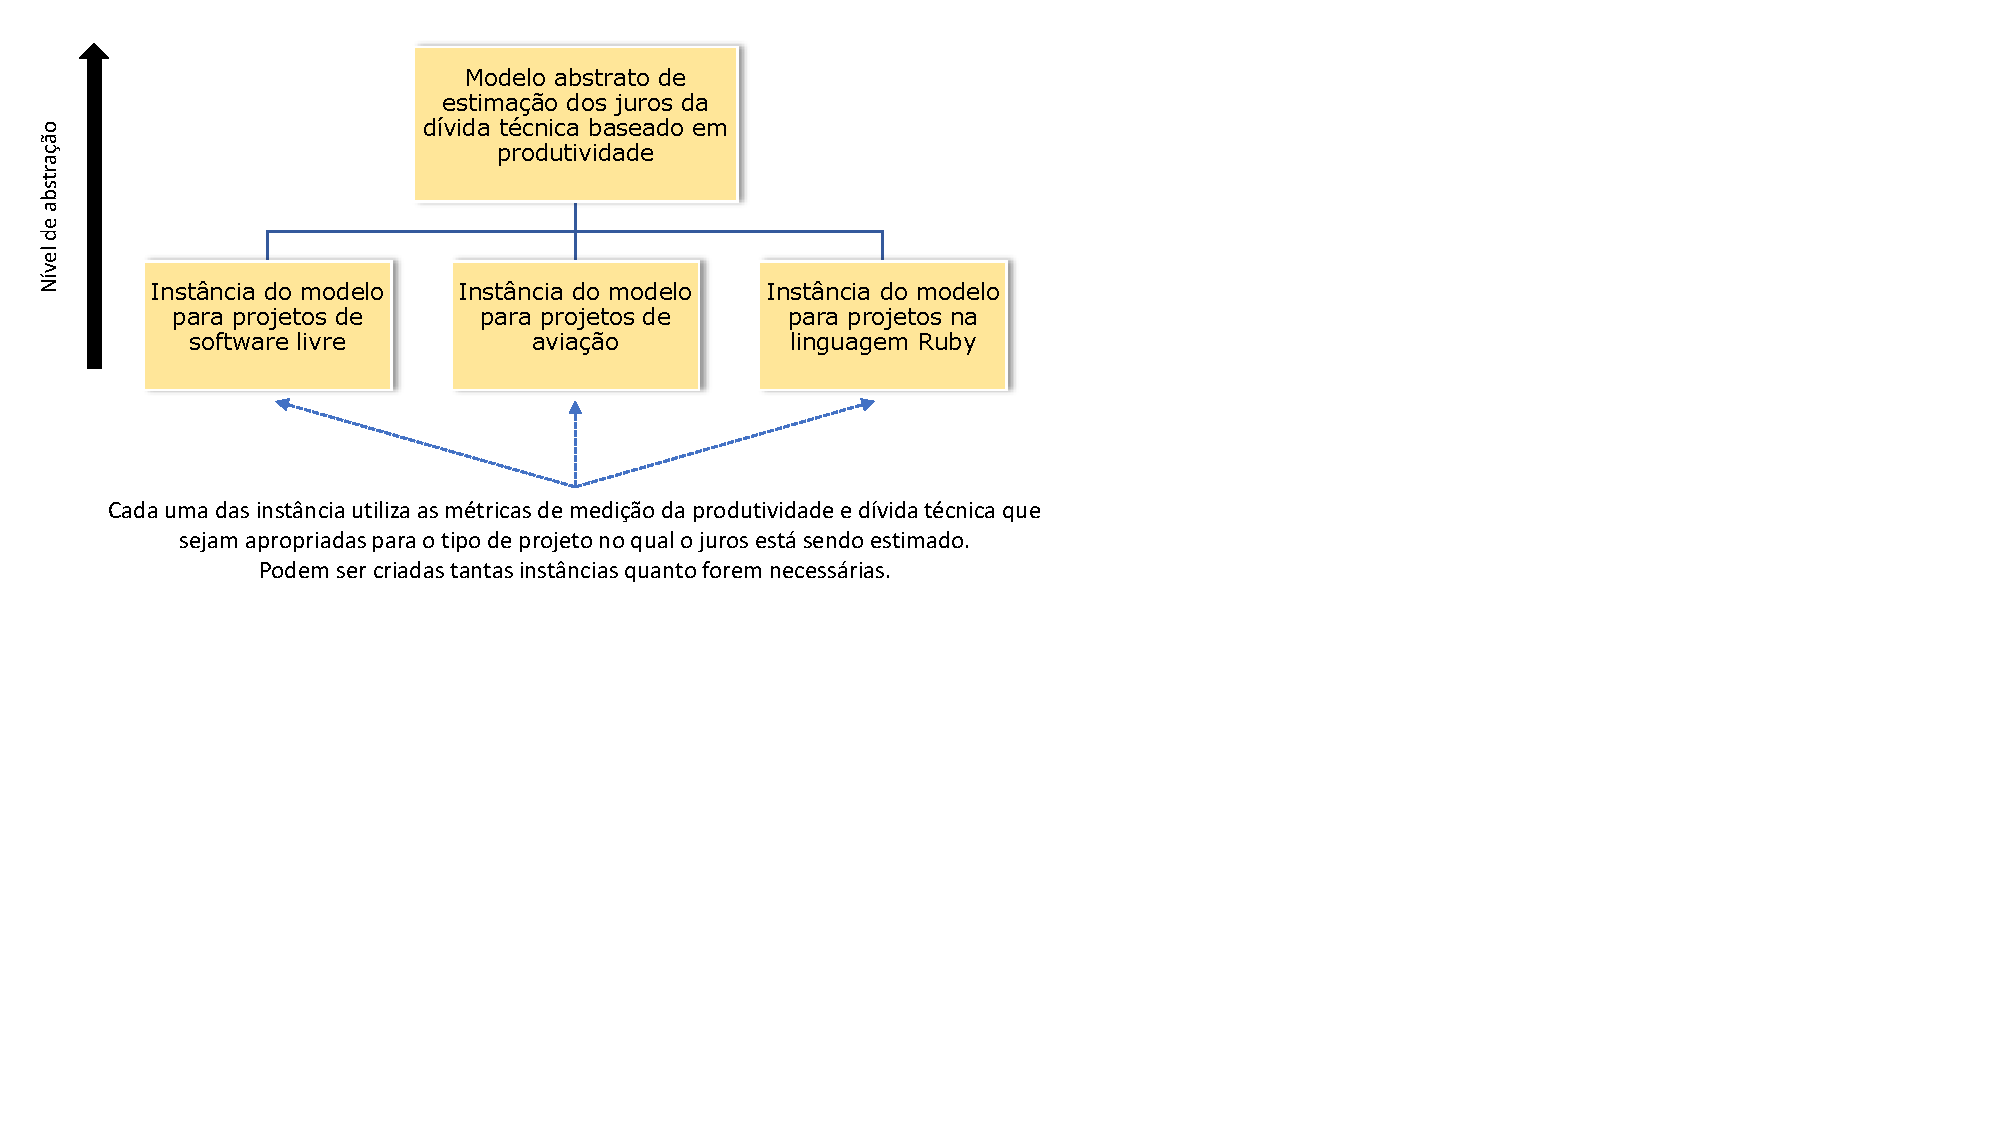
\includegraphics{capitulo_metodo/NiveisDeAbstracoesModelo.pdf} 
  \caption{Níveis de abstração do modelo es estimação dos juros da dívida técnica. }
  \label{fig:cap_metodo_niveis_abstracao} 
\end{figure}




\section{Pesquisa quantitativa}




De acordo com Creswell\cite{w2016research}, uma pesquisa quantitativa tem como foco principal a quantificação de relacionamentos ou a comparação de um ou mais grupos. Adicionalmente, conforme explicado por Wohlin et al.\cite{wohlin2003empirical}, as pesquisas quantitativas são apropriadas quando existe a necessidade de testar o efeito de alguma atividade ou manipulação. Segundo Wang at al. \cite{wang201331}, a abordagem quantitativa disponibiliza uma série de ferramentas para descobrir, com um determinado nível de confiança, a verdade a respeito de um objeto de estudo. O que difere substancialmente uma pesquisa quantitativa de outra qualitativa é seu grau de  objetividade a respeito dos fenômenos avaliados. Na abordagem quantitativa há pouco ou nenhuma margem para que haja, durante o processo de coleta de dados, uma interpretação dos indivíduo relacionados com o evento analisado. Ao invés disso, são utilizados apenas fatos que não dependem de sensações, reflexões, intuições ou qualquer outra forma subjetiva de avaliação. Isso faz com que os dados numéricos sejam predominantes em pesquisas quantitativas.  Essa característica permite que, utilizando poucos recursos, um grande volume de dados possam ser coletados e analisados.  Amaratunga et al. \cite{amaratunga2002quantitative} lista algumas das principais características de uma pesquisa quantitativa:

\begin{itemize}
\item Permitem a replicação e a comparação de resultados.
\item Indepedência entre o observador e o objeto observado.
\item A confiabilidade e validade dos resultados podem ser determinadas de forma mais objetiva.
\item Enfatiza a necessidade de formular hipóteses para subsequentes verificações.
\end{itemize}

São muitas as atividades necessárias para a realização de uma pesquisa quantitativa. Essas atividades podem ser dividas em duas fases. A primeira fase é constituidas por atividades de planejamento, obtenção e validação dos dados necessários para a avaliação do objeto da pesquisa. Esses dados podem ser obtidos de diversas formas. As mais comuns são a realização de questionário, experimentos, estudos de caso e, mais recentemente, a mineração de repositórios. A segunda fase consiste na avaliação desses dados utilizando métodos matemáticos, estatisticos ou computacionais.  

Conforme argumentado por Brown, N et al.\cite{brown2010managing}, há uma predominância na utilização de métodos qualitativos nas pesquisas a respeito da dívida técnica e isso pode levar a conclusões baseadas em intuições atraentes, porém não necessariamente corretas. Essas conclusões incorretas podem ser explicadas pela existência de dados obtidos por meio de declarações imprecisas. Essas declarações podem ser dadas pela dificuldade que as pessoas envolvidas com os projetos de software têm em assumir suas deficiências ou falhas. Por isso, Brown, N et al.\cite{brown2010managing} indica a necessidade da criação de modelos baseados em abordagens quantitativas para viabilizar a criação de rigorosas técnicas de gerenciamento da dívida técnica que possam ser aplicadas em projetos de larga escala. Neste trabalho iremos propor um modelo para estimação da dívida técnica. Para analisarmos a validade desse modelo, iremos realizar um estudo de caso quantitativo utilizando dados de projetos de software hospedados na plataforma GitHub. 

\section{Estudo de caso}

 De acordo com Wohlin et al.\cite{wohlin2003empirical}, um estudo de caso é um método de pesquisa onde são utilizados dados de situações reais. Diferentemente de um experimento, no estudo de caso o pesquisador tem menos ou nenhum controle sobre os acontecimentos.  No contexto de projetos de software, um estudo de caso tem como objetivo monitorar as atividades realizadas durante o projeto. Segundo Yin, Robert K\cite{yin2011applications}, existem dois tipos de estudo de caso: os únicos e os múltiplos. Os estudos de casos únicos são aqueles onde os dados são obtidos de um único ``caso'',  que pode ser um projeto, uma empresa, um indivíduo ou qualquer outra unidade que seja apropriada para o estudo do objeto da pesquisa. Por outro lado, um estudo de caso múltiplo envolve diferente unidades de interesse. Ou seja, são consideras diversas empresas, projetos, indivíduos e etc. É preferível a realização de estudos de caso múltiplos já que os mesmos facilitam a generalização dos resultados obtidos por fornecerem multiplas visões a respeito do objeto de pesquisa. Tendo isso em vista,  para avaliarmos o modelo de estimação do comportamento dos juros da dívida técnica descrito no capítulo \ref{estimacao:juros}, realizaremos um estudo de caso multiplo envolvendo milhares de projetos armazenados em um repositórios de software.

\subsection{Etapas do estudo de caso}



 O estudo de caso será realizado em 5 etapas conforme resumido na  Figura \ref{fig:cap_metodo_resumo_etapas}.  Foi desenvolvida  uma ferramenta para automatizar grande parte das atividades realizadas em cada etapa. Mais detalhe sobre a ferramenta de apoio serão fornecidos na seção \ref{cap_estudo_caso_ferramenta}. 
 
\label{sec:Passos_Elaboracao_Modelo}

  \begin{figure}[H]
  \centering
  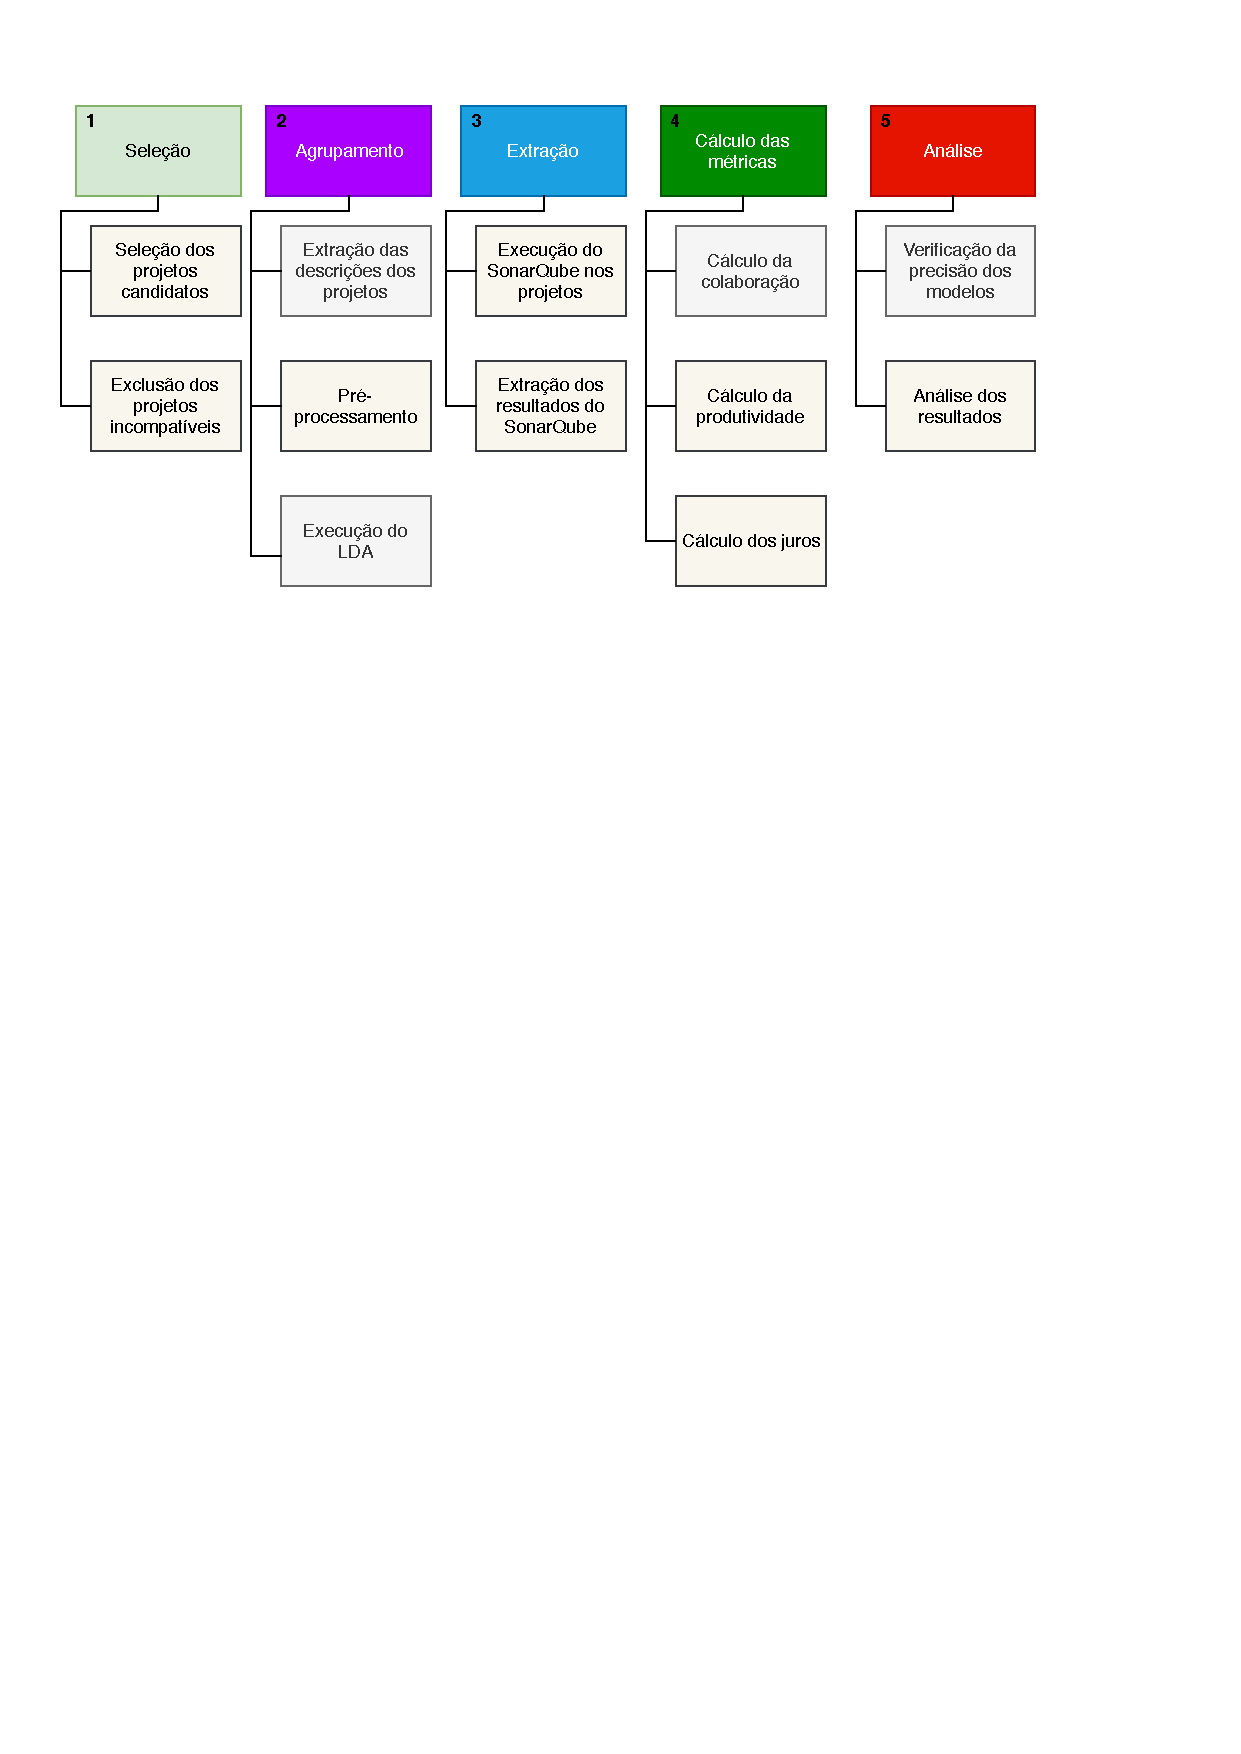
\includegraphics{capitulo_metodo/ResumoEtapas.pdf} 
  \caption{Resumo das etapas do estudo de caso. }
  \label{fig:cap_metodo_resumo_etapas} 
\end{figure}

\subsection{Etapa 1 - Seleção dos projetos} 


Foram usados diversos critérios para selecionar os projetos incluídos no estudo de caso. Os primeiros deles estão relacionados com a necessidade de verificar se um repositório presente no GitHub realmente se trata de um projeto de software. Isso é necessário já que por disponibilizar a possibilidade de gratuitamente armazenar arquivos, muitas vezes o Github é utilizado para armazenar conteúdo que não é um projeto de software. É comum encontrar arquivos de sites, exercícios escolares, contratos e diversos outros itens que não têm relação com o objeto desta pesquisa. Na literatura, são encontradas pesquisas que fornecem heurísticas para identificar se um repositório no GitHub é um projeto de software ou não. Um exemplo é  o trabalho de Kalliamvakou et. al.\cite{kalliamvakou2014promises} onde são elencados diversos perigos encontrados na mineração de dados no GitHub. Outro trabalho relevante é o de Russel. M.\cite{russell2013mining} onde o autor faz um abrangente análise a respeito da mineração de dados no Github como também em diversas outras plataformas. 


\subsection{Etapa 2 - Agrupamentos dos projetos semelhantes}

Primeiramente, iremos encontrar e agrupar versões de diferentes projetos que apresentam similaridades contextuais e contenham instâncias dos tipos de dívida técnica que iremos analisar nesta pesquisa. A similaridade entre os projetos será definida seguindo técnicas encontradas na literatura. Algumas técnicas candidatas são as de Idri. A., et. al. \cite{idri2001fuzzy}, Yamamoto. T., at. al. \cite{yamamoto2005measuring}, Park. S. et. al. \cite{park2012similarity}.

Os grupos de projetos serão formados observando as seguintes regras:
\begin{enumerate}
\item Possuam uma versão que tenha uma das dívidas técnicas que será analisadas neste estudo. A lista de dívidas técnicas está descrita na tabela \ref{table:tiposDivida}. Haverá um grupo para cada tipo de dívida técnica. 
\item Sejam similares de acordo com a técnica de definição de similaridade que será escolhida posteriormente.
\end{enumerate}

Ao final desta etapa, haverá um conjunto de grupos de projetos. Cada grupo irá conter apenas projetos similares e no qual tenha sido encontrado um determinado tipo de dívida técnica em uma de suas versões. Na tabela \ref{table:exemploGrupos} podemos observar alguns exemplos de grupos. Nos exemplos dados, é possível ver que os projetos 1 - 2 e 3 - 4 estão em grupos diferentes, ainda que a dívida técnica que eles contenham seja do mesmo tipo. Isso pode acontecer caso haja uma diferença entre as propriedades do projeto. Por exemplo, os projetos 1 e 2 podem ser muito maiores que os projetos 3 e 4. Dessa forma, faz mais sentido comparar os efeitos dos juros da dívida técnica apenas entre os projetos 1 - 2  e 3 - 4 em vez de comparar com os projetos 1,2,3 e 4. 





\subsection{Etapa 3 - Extração dos dados}

Nesta fase iremos particionar cada um dos grupos de forma a separar os projetos que em algum momento corrigiram a dívida técnica e os que não corrigiram. Esse particionamento será feito analisando as futuras versões do software. Caso, em um grupo, alguma das partições fique vazia, o grupo será descartado. Na tabela \ref{table:exemploGrupos} podemos ver os campos versão da dívida e versão da solução. Esses campos armazenarão o número da versão do software onde a dívida foi criada e o número da versão onde ela foi corrigida, caso tenha sido corrigida. 



\subsection{Etapa 4 - Cálculo das métricas de produtividade}


\subsection{Etapa 5 -Análise dos resultados}

 Nesta etapa, iremos realizar uma análise estatística dos dados obtidos nas etapas anteriores. Para tal, utilizaremos técnicas da estatística inferencial e métodos da inteligência artificial. Os objetivos nessa etapa são identificar padrões no comportamento dos juros da dívida técnica e na variação de esforço encontrados entre os projetos dos grupos que resolvem a dívida técnica e os que não resolvem. Pretendemos utilizar métodos estatísticos para avaliar o grau dessa variação e a sua significância. 









\begin{figure}[h]
  \centering
  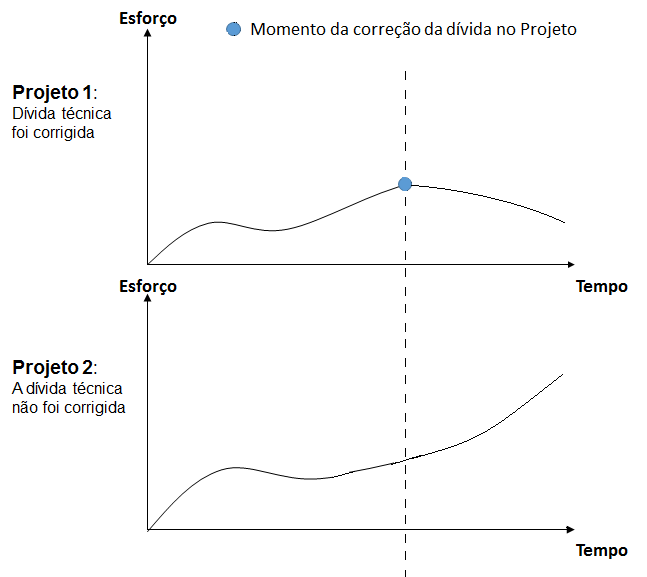
\includegraphics[width=17.12cm,height=15.26cm]{diferenca_projetos.png} 
  \caption{Representação da variação de esforço entre projetos que resolveram a dívida técnica e os projetos que não resolveram. }.
  \label{fig:variacao_projetos} 
\end{figure}








\subsubsection{Etapa 5 -Elaboração do modelo de estimação}
\label{sec:analise_dados_modelo}

Finalmente, para responder as questões de pesquisa definidas no capítulo \ref{cap:objetivos}, iremos elaborar um modelo de estimação dos juros da dívida técnica. Esse modelo será elaborado usando as informações sobre a evoluçao dos juros da dívida técnica em projetos hospedados no GitHub. Ou seja, o modelo compreende tanto as estratégias de identificação da correção das dívidas técnicas quanto as formas de avaliação do esforço adicional causados por elas.   Por meio deste modelo, será possível identificar qual o esforço adicional esperado para o projeto devido a existência de um determinado tipo de divida técnica. Consequentemente, será possível identificar quais dívidas técnicas geram mais juros.

Uma das características desejadas para esse modelo é a possibilidade de que ele possa ser extendido.  A medida que novas formas de identificação da dívida técnica sejam implementadas, novos tipos de dívida técnica poderão ser analisadas. Outra possibilidade, será a inclusão do modelo em ferramentas de desenvolvimento de software. Apesar de não ser um dos objetivos desta pesquisa, o modelo será elaborado de forma que possa ser incorporado futuramente em ferramentas de desenvolvimento e assim poder ser utilizado em situações reais.





\begin{figure}[!h]
  \centering
  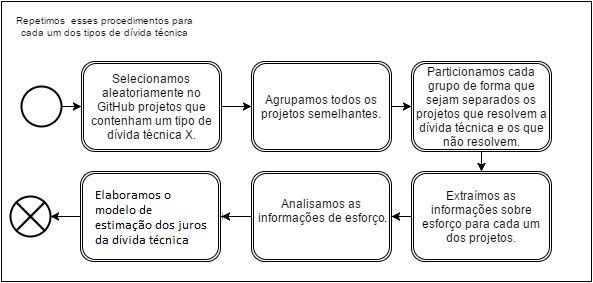
\includegraphics[width=15.69cm,height=7.49cm]{resumo_metodo.png} 
  \caption{Resumo do processo de extração de dados. }.
  \label{fig:resumo_metodo} 
\end{figure}




\begin{table}[!h]

\caption{Exemplos da divisão dos projetos em grupos}
\label{table:exemploGrupos}
\def\arraystretch{1.1}%
\begin{tabular}{|l|l|l|l|l|l|}
\hline
Projeto   & Ver. da dívida & Ver. da solução & Dívida técnica                     & Grupo & Particao      \\ \hline
Projeto 1 & 1.0              & 3.5               & God Class                          & G1    & Resolvido     \\ \hline
Projeto 2 & 2.4              & -                 & God Class                          & G1    & Não resolvido \\ \hline
Projeto 3 & 3.5              & 7.5               & God Class                          & G2    & Resolvido     \\ \hline
Projeto 4 & 3.8              & -                 & God Class                          & G2    & Não resolvido \\ \hline
Projeto 5 & 8.9              & 10.5              & Complex. Ciclomática Excessiva & G3    & Resolvido     \\ \hline
Projeto 6 & 4.6              & -                 & Complex. Ciclomática Excessiva & G3    & Não resolvido \\ \hline
\end{tabular}
\end{table}


 

\section{Método de avaliação}



Utilizaremos nesta pesquisa as informações dos projetos de software hospedados na plataforma GitHub. Esse sistema contém uma imensa quantidade de projetos e usuários. Se por um lado o GitHub apresenta uma quantidade e variedade de projetos, por outro não contém informações sobre o esforço que foi gasto para o desenvolvimento dos projetos nela hospedados. Essa informação poderia ser utilizada para medir os juros da dívida técnica mais diretamente ao invés da abordagem indireta descrita na seção \ref{sec:Passos_Elaboracao_Modelo}. Para realizarmos uma validação em relação aos resultados obtidos nesta pesquisa, iremos utilizar outros repositórios de software menores, porém que possuem informações detalhadas sobre os recursos utilizados durante os projetos. Iremos selecionar aleatoriamente alguns dos projetos nesses repositórios que possam ser agrupados de acordo com os procedimentos da seção \ref{sec:Passos_Elaboracao_Modelo}. Então iremos extrair as informações sobre o juros da dívida técnica e realizar as mesmas análises descritas na seção \ref{sec:analise_dados_modelo}. Por fim, iremos comparar os resultados obtidos com os dados provenientes do GitHub com os dados vindos dos repositórios menores e com informações de utilização de recursos. Essa triangulação de resultados permitirá uma maior confiança em relação aos resultados obtidos nesta pesquisa. 








